\section{IoTDSL}
\label{sec:IoTDSL}

Based on the challenges identified in Section~\ref{sec:Motivation}, we now introduce \IOTDSL, our \DSL devoted to facilitate the high-level manipulation of \IOT systems. At the heart of \IOTDSL are two governing principles. First, we promote a clean separation of concerns for all aspects the \DSL has to handle, by specifying one sublanguage for each concern. We believe this approach to be scalable, and to support independent evolutions of each concern without impacting the other aspects, since those aspects are composed through well-defined interfaces. Second, our \DSL relies on events, a natural paradigm for specifying various models of interactions that is widely used in embedded and critical systems, and where a clear separation between the system and its environment is performed, further empowering the separation of concerns. Despite its early stage of development, \IOTDSL shows its ability to capture the definition of small-scale \IOT systems appropriately.

Building a well-calibrated \DSL is known to be difficult and error-prone. It usually requires a broad expertise of the domain under consideration before a consensus emerges on the domain's key concepts and how to effectively represent them. Fortunately, \MDE technologies operated substantial breakthrough over the past decade, allowing language designers to define their own \DSL structures and user interfaces more easily. Adopting such a trend, we have built an early prototype for our \DSL under GeMoC \cite[\url{http://gemoc.org}]{bousse-16}, a \MDE framework that supports both visual and textual representations as concrete syntaxes and maintains a full synchronisation between them. Since we are at early development stage, only a textual syntax is currently available to modellers, but other syntaxes, even graphical ones, can be smoothly added thanks to \textit{GeMoc}.

To illustrate our proposal, we show how \IOTDSL is built by describing each sublanguage, following the \DSL components identified in Section \ref{sec:Motivation-Components}, and illustrate them by providing the full implementation for Alice's apartment as depicted in Section \ref{sec:Motivation-Scenarios}.

\begin{figure*}%
  \centering  
  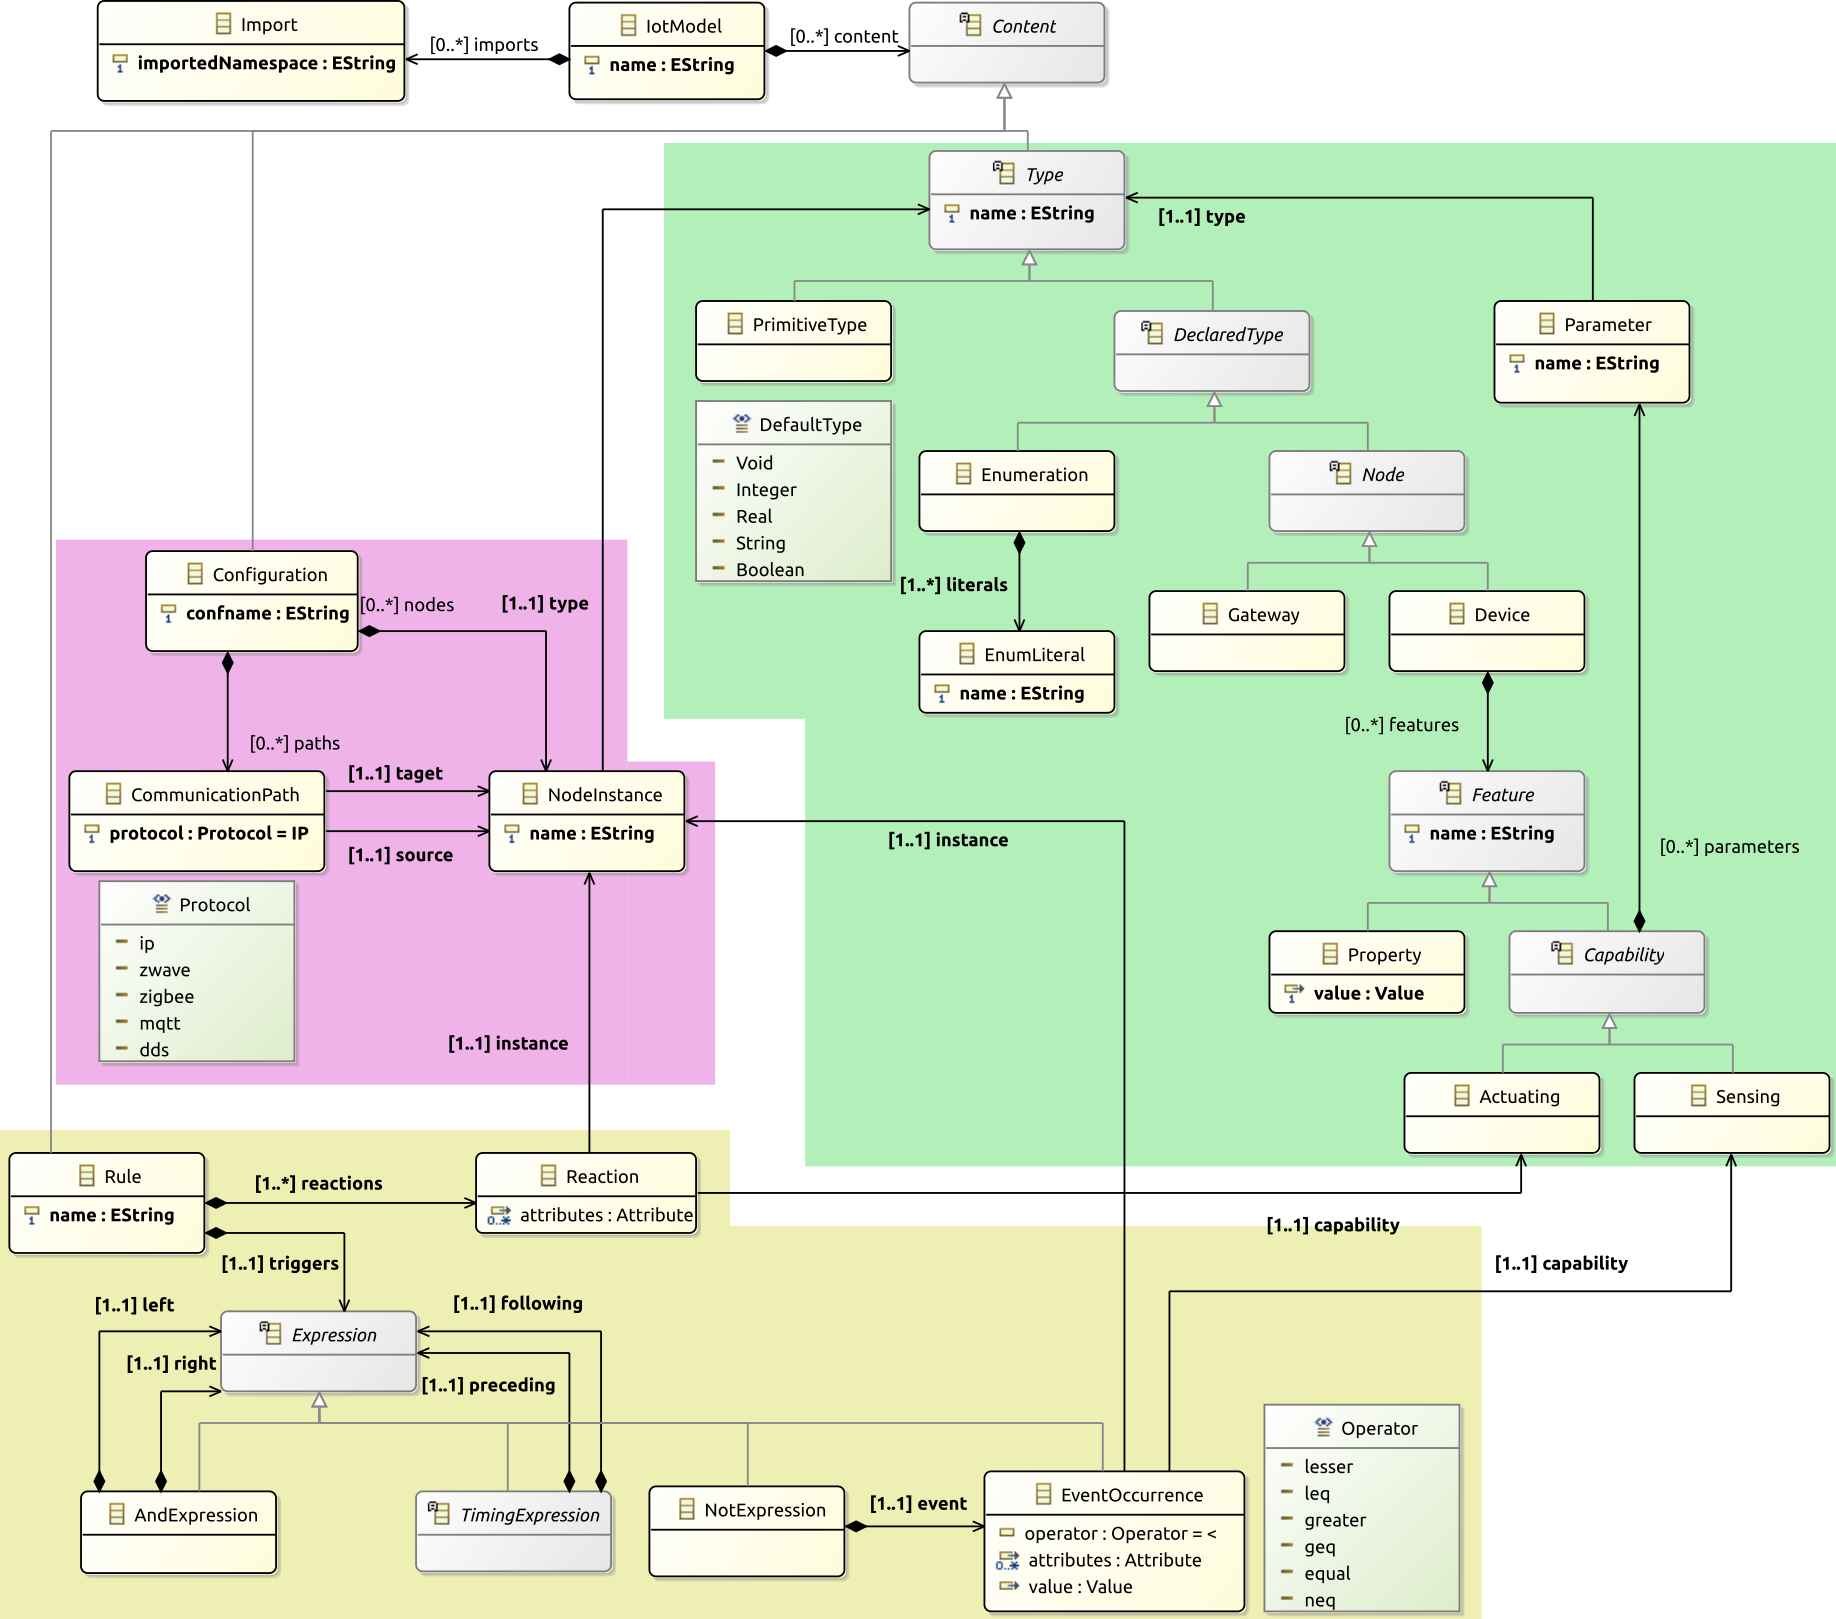
\includegraphics[width=.98\linewidth]{iotdsl-metamodel}%
  \caption{Metamodel of \IOTDSL, separated in three concerns: \emph{Type Definition} captures devices' capabilities (top-right green part), \emph{Network Configuration} details how device instances are connected to each others (middle-left purple part), \emph{Business Rules} defines the functionalities expected from the IoT installation (bottom yellow part).}%
  \label{fig:IoTDevice-MM}%
\end{figure*}

\subsection{Type Definition}
\label{sec:IoTDSL-TD}

The first task is to provide a description of which capabilities each device included in the \IOT system possess: how each device may provide information about the environment through a \emph{sensing} operation; and how it could react and influence it through \emph{actuations}. Our framework currently requires that an advanced user that is able to reason properly about how to effectively manipulate a device and extract the relevant information, but is flexible enough to accomodate automation in the future, so that information about devices could be automatically extracted from pre-existing devices databases (either from a knowledge database the \IOT system is connected to, or from a library of \emph{off-the-shelf devices}).

%In this section, we define \IOT devices' types, \textit{i.e.} which capabilities are available to the users in terms of getting information from the environment, \textit{a.k.a.} sensing, and operating on the environment, \textit{a.k.a} actuating. In our framework, type definitions either come from an advanced user who is able to reason properly about a particular device and extract the relevant information, or from a pre-existing devices database, either being a repository the system is connected to, or a library of \textit{devices-off-the-shelf}. 

\begin{figure*}%
  \centering  
  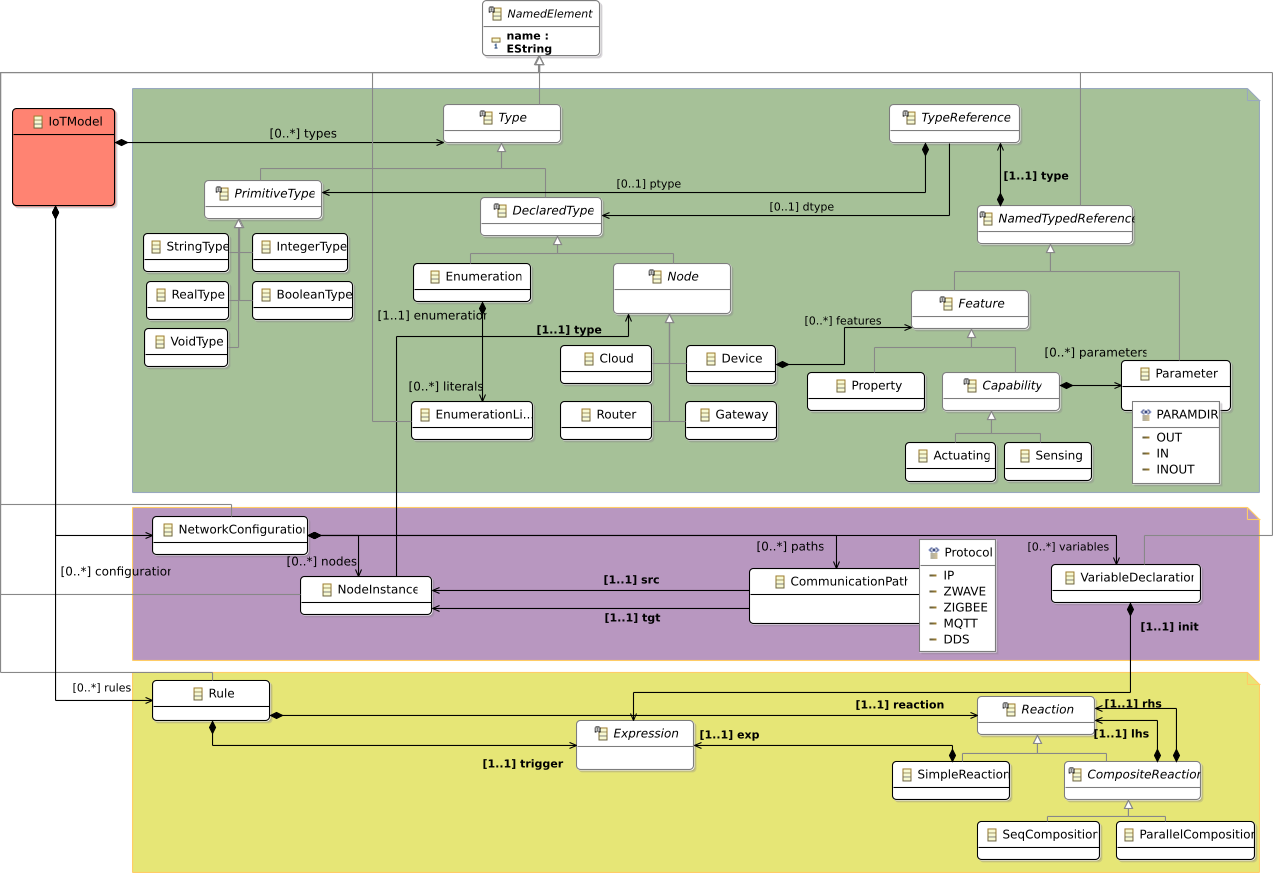
\includegraphics[width=.92\linewidth]{IoTDevice-MM.png}%
  \caption{Metamodel of \IOTDSL, separated in three concerns: \emph{Type Definition} captures devices' capabilities (top green part), \emph{Network Configuration} details how device instances are connected to each others (middle purple part), \emph{Business Rules} defines the functionalities expected from the IoT installation (bottom yellow part).}%
  \label{fig:IoTDevice-MM}%
\end{figure*}

The concepts dedicated to type definition are shown in Figure~\ref{fig:IoTDevice-MM} (green background). This part is similar to the notion of \textsf{Classifier} in \textsc{Mof}-like languages: a \textsf{Type} is either a \textsf{PrimitiveType}, or a user-defined \textsf{DeclaredType}. We distinguish between general \textsf{Gateway}s, which centralise information and processing, and \textsf{Node}s deployed in the environment and communicating with gateways, and which possess capabilities to interact with the environment. A \textsf{Capability} is basically a parameterised event that drives the node to either capture data from the environment, to act on it, or to perform both. This abstract view of an ``thing'' allows us to manipulate any device at a high abstraction level, exhibiting a clean and uniform interface for end-users based on device capabilities. Since \textsf{Node}s are \textsf{Type}s themselves, it remains possible to reference them as a parameter for the purpose of dynamic discovery across devices.

Listing~\ref{lis:RE-TypeDeclarations} illustrates how the devices in Figure~\ref{fig:scenario} are declared in \IOTDSL. Each device is introduced by the keyword \textsf{device}, possesses a name and lists capabilities that correspond to reporting events (\textsf{sensing}) or operating over the environment (\textsf{actuating}). 

\begin{table}
	\begin{minipage}[b]{.45\textwidth }%
		\begin{lstlisting}[language=iotdsl]	
gateway Middleware
device DoorDetector {
	sensing opened()
	sensing closed()
}
device MotionDetector {
	sensing moving()
}
device ToggleSwitch {
	sensing toggle()
}
		\end{lstlisting}
	\end{minipage}\hfill%
	\begin{minipage}[b]{.45\textwidth}
		\begin{lstlisting}[language=iotdsl, firstnumber=12]
		
device LightSensor {
	sensing light()
}
device LightBulb {
	actuating on()
	actuating off()
}	
device Alarm {
	actuating sound()
}
		\end{lstlisting}
	\end{minipage}
	\caption{Type declarations in \IOTDSL: capabilities as high-level events.}
	\label{lis:RE-TypeDeclarations}
\end{table}

Any IoT system should declare a special device, introduced with the keyword \textsf{gateway}, that centralises data from all devices connected to it, as we will show in Section \ref{sec:IoTDSL-NetworkConfiguration}. This device will be responsible of the event orchestration and will host the \CEP engine that embeds the implementation of the business rules. Also note that the above model is the \textit{user-defined} part of \IOTDSL. In the background, abstract events attached to all devices will need to be mapped to concrete low-level \textsc{Api}s events using a dedicated mapping language that is out of the scope of this paper.


\subsection{Network Configuration}
\label{sec:IoTDSL-NetworkConfiguration}

The configuration constructs of \IOTDSL are specified in the middle-left purple part of Figure~\ref{fig:IoTDevice-MM}. Since we use an architecture centralised around gateways, a network \textsf{Configuration} is a graph-like structure where vertices are \textsf{Gateway}s and \textsf{NodeInstance}s (so that instances may communicate with each others), while edges represent \textsf{CommunicationPath}s (or channels). Such paths define, among others, one or more protocols used to interact. We actually rely on existing platforms, such as OpenRemote (\url{http://www.openremote.org}) or SmartThings ({\url{https://www.smartthings.com}) to handle the intricate details of the protocols since such details are, from an end-user point of view, technical aspects rather than essential matters of the configuration itself. By knowing which protocols are used between each pair of devices, we can automatically perform data conversion in the proper format required by the protocols: most of those protocols are already implemented in \textit{General-Purpose Programming Languages} (\textsc{Gpl}s), like Java or C.

Listing~\ref{lis:RE-Network} shows an instantiation as well as the connection that conforms to the types given in Listing~\ref{lis:RE-TypeDeclarations} and the configuration presented in Figure~\ref{fig:scenario}.
	
	
\begin{table}
	\begin{minipage}[b]{.45\textwidth }%
		\begin{lstlisting}[language=iotdsl]	
configuration SmartHouse {
	node middle   		   : Middleware
	node alarm					 : Alarm
	node toggle          : ToggleSwitch
	node frontDoor			 : DoorDetector
	node parentDoor			 : DoorDetector
	node childDoor			 : DoorDetector
	node balconyDoor 		 : DoorDetector
	node outLight				 : LightSensor
	node livingLight		 : LightSensor
	node livingBulb			 : LightBulb
	node bathroomBulb    : LightBulb
	node foyerBulb       : LightBulb
	node balconyMotion	 : MotionDetector
	node foyerMotion  	 : MotionDetector
	node hallMotion	     : MotionDetector
		\end{lstlisting}
	\end{minipage}\hfill%
	\begin{minipage}[b]{.45\textwidth}
		\begin{lstlisting}[language=iotdsl, firstnumber=17]
	from alarm			   to middle via IP
	from frontDoor 	   to middle via IP
	from parentDoor    to middle via IP
	from childDoor     to middle via IP
	from balconyDoor   to middle via IP
	from outLight      to middle via IP
	from livingLight   to middle via IP
	from livingBulb    to middle via IP
	from bathroomBulb  to middle via IP
	from foyerBulb     to middle via IP
	from balconyMotion to middle via IP
	from foyerMotion   to middle via IP
	from hallMotion    to middle via IP
}
		\end{lstlisting}
		\vspace*{.3cm}
	\end{minipage}
	\caption{Network Configuration in \IOTDSL for our smart house.}
	\label{lis:RE-Network}
\end{table}
	
A specific device is considered as an instance of a defined type such that particular devices with the same set of capabilities may be distinguished via identifiable unique references. Communications are purely declarative and only mention the protocol type (introduced by the \texttt{\color{codeviolet}{\textbf{via}}} keyword). In our example, we simply decided to use an \textsf{IP} protocol for all bindings. Note that a similar mapping process that the one described at the end of Section~\ref{sec:IoTDSL-TD} is required to reify abstract connections between \textsf{NodeInstances} to physical ports and protocols, but again, these mapping statements are outside of the scope of this paper. 


\subsection{Business Rules}
\label{sec:IoTDSL-BusinessRules}

Business rules are the core of the manipulation of \IOT systems and compose the third part of \IOTDSL as detailed in the bottom yellow part of Figure~\ref{fig:IoTDevice-MM}. This last sub-language relies on an event-based framework that allows to specify a set of \textsf{Rule}s expressing the many functionalities an end-user wants to achieve in his/her concrete configuration. 

An \IOTDSL Business Rule is identified by the keyword \textsf{rule} followed by an unique identifier, and a body of the form << \texttt{\textbf{\color{codeviolet}{when}} trigger \textbf{\color{codeviolet}{do}} reaction} >>. Rules' \texttt{trigger}s are cyclically evaluated against the surrounding environment and specify the conditions under which the corresponding \texttt{reaction}s have to be performed to realise the end-users' scenarios. A \texttt{reaction} defines actuations on the \IOT system to send or require data of identified devices, or issues events that are internally used to synchronise rules. 

%must be triggered. Rules' \textsf{trigger}s are cyclically evaluated against the surrounding environment and a \textsf{reaction} defines a sequential or parallel combination of capabilities, enabling to sort actions by, or require data from some identifiable devices. Inside the \textsf{trigger}, users typically check events to evaluate their presences, but as we will see in the following examples, they are also able to check on their absence or returned values. A typical \textsf{reaction} may be to switch on all lights in a house, or only the ones of a certain type by sending new events.

Our approach is currently purely middleware-oriented: all rules are evaluated inside a single gateway that supposedly possesses enough processing power. We leave as future work the exploration of parallelisation techniques to support multiple gateways that communicate appropriately, or the possibility to decentralise parts of the computation into nodes with sufficient processing and power resources to optimise resource consumption and lighten communication exchanges. 

We now illustrate how the scenarios Alice is concerned about (cf. Section \ref{sec:Motivation-Scenarios}) can be translated into business rules in \IOTDSL with the devices' definitions detailed in Listings~\ref{lis:RE-TypeDeclarations} and \ref{lis:RE-Network}. 

\begin{description}[leftmargin=0cm]
	\item[Switching entrance lights on when coming in]  When Alice gets home (and thus opens the front door), she wants the lights to be automatically switched on in the foyer and in the living room.
	\begin{lstlisting}[language=iotdsl,
							label=lis:home-rule,
		caption=Rule to switch on the lights at home incoming]
rule SwitchLightsWhenEntering:
	when (foyerMotion.moving after frontDoor.opened) do {
		foyerBulb.on
		livingBulb.on
	}
	\end{lstlisting}
	This rule introduces what we call \emph{facilitators}, i.e. keywords that define an unspecified time window in which a sequence of events should be observed. This time window is system-specific and needs to be defined independently in configuration files independent of descriptions in \IOTDSL. In this case, the \inlineI{foyerMotion} should detect movement \emph{nearly after} the \inlineI{frontDoor} detects an opening. 
		
	Note that reactions are defined as a sequence that does not matter: the order in which the \inlineI{foyerBulb} and the \inlineI{livingBulb} switch on largely depends on the platform capacities, i.e. they can be actuated synchronously or sequentially (in which case, no guarantee is given that the definition order will be respected). At the abstraction level \IOTDSL operates, it is irrelevant since the end user wishes to see both switched on at some point, without having to consider low-level details that would enforce such behaviour.

	\item[Illuminate bathroom when children wake up at night] When Alice's little boy wakes up at night, she would like to have the light in the bathroom to be switched on to prevent him from falling or injuring himself. Analogously, she wants the light to be switched off when he gets back to sleep afterwards.
	\begin{lstlisting}[language=iotdsl,
							label=lis:night-rule,
		caption=Rules to switch on\//off lights in the corridor at night]
rule SwitchBathroomLightOnAtNight:	
	when (not livingLight.light and 
	 (hallMotion.moving after childDoor.opened)) do {
		bathroomBulb.on
	}

rule SwitchBathroomLightOffAtNight:	
	when (not hallMotion.moving within 3 min from childDoor.closed) do {
		bathroomBulb.off
	}
	\end{lstlisting}
	The rule \inlineI{SwitchBathroomLightOnAtNight} introduces a new keyword \inlineI{not}, which represents the \emph{absence} of a certain event type, here \inlineI{livingLight.light}. This is different than simply observing some events occuring. Note also that the second part of the rule trigger uses parenthesis to relate the facilitator \inlineI{after} to the closest event \inlineI{childDoor.open}, instead of spanning on the whole condition.

	The rule \inlineI{SwitchBathroomLightOffAtNight} presents a combination of negation with an explicit time window with the construct \inlineI{within ... from}: it indicates that no event of type \inlineI{movement} from the hall motion sensor should occur in a three-minute time window after observing the \inlineI{closed} event from the boy's door, in order to trigger the rule. \IOTDSL defines several useful time units to cope with simpler definitions (seconds, minutes, hours, or a combination of the three). 
	

	\item[Report unsupervised children on balcony] Alice considers that it is a critical situation if a child enters into the balcony without her knowledge, because of fall risks. To avoid that, she placed a switch button high enough that only an adult could press when accompanying a child outside. If the button is not pressed within 3 seconds after someone enters the balcony, an alarm should sound.
	\begin{lstlisting}[language=iotdsl,
							label=lis:balcony-rule,
		caption=Rules to sound the alarm in case of an unsupervised child on the balcony]
rule AlarmWhenChildOnBalcony:	
	when (not toggle.toggled within 5 sec from 
			(balconyMotion.moving after balconyDoor.opened)) do {
		alarm.sound
	}
	\end{lstlisting}
	This last rules states that once the balcony door has been opened and movements are detected on the balcony, the alarm should sound unless the toogle button is pressed in a five-second time window. This rule is similar to \inlineI{SwitchBathroomLightOffAtNight}, except that the baseline of the time window is here a composite event using a facilitator: once an opening followed by movements on the balcony is observed, we expect the toggle button to be pressed. 
\end{description}

To summarise, an end-user uses the Business Rules sublanguage to specify the scenarios of interest in the form of \inlineI!when (trigger) do {actuations}!: the \inlineI{trigger} condition specifies the event (non-) occurrence pattern under which the \inlineI{actuations} are performed, by using common boolean connectors as well as time windows to observe delayed events; whereas the \inlineI{actuations} are undeterministically performed independently to their definition order. 

From a qualitative point of view, adopting a rule-based language presents the advantage of mimicking the cognitive process of establishing a scenario, which should ease the adoption of \IOTDSL. However, we are conscious that this requires a further examination and actual validation with end-users that are not aware of the underlying \DSL mechanisms, but we believe that presenting a visual representation for rules and powerful analysis of rule activation could ease the adoption process and facilitate scenario definitions.






